\documentclass[letterpaper]{scrreprt}

%% Language and font encodings
\usepackage[spanish]{babel}
\usepackage[utf8]{inputenc}
\usepackage[T1]{fontenc}

\usepackage{pdfpages}
%% Sets page size and margins
\usepackage[letterpaper,top=3cm,bottom=2cm,left=3cm,right=3cm,marginparwidth=1.75cm]{geometry}

%% Useful packages
\usepackage{amsmath}
\usepackage{graphicx}
\usepackage[colorinlistoftodos]{todonotes}
\usepackage[colorlinks=true, allcolors=black]{hyperref}

\usepackage{geometry}
\usepackage{xcolor}
\definecolor{titlepagecolor}{cmyk}{0,.84,.80,.19}
\definecolor{namecolor}{cmyk}{1,.50,0,.10} % Here
\setlength{\parindent}{4em}
\setlength{\parskip}{1em}
\renewcommand{\baselinestretch}{1.5}

\title{Snake 3D}
\subtitle{Diseño del Sistema}
\author{Mateo Florido Sanchez}


\graphicspath{{Figures/}}

\begin{document}
% ----------------------------------------------------------------
\begin{titlepage}
	\newgeometry{left=7.5cm}
	\pagecolor{titlepagecolor}
	\noindent
	
\includegraphics[width=4cm]{Extras/javeriana.png}\\[-1em]
	\color{white}
	\makebox[0pt][l]{\rule{1.3\textwidth}{1.5pt}}
	\par
	\noindent
	\textbf{\LARGE \textsf{Snake 3D - Documento Diseño de Sistema}}
	\vfill
	\noindent
	{\huge \textsf{Versión 1.0}}
	\vskip\baselineskip
	\noindent
	\textsf{Agosto 2019}
\end{titlepage}
\restoregeometry % restores the geometry
\nopagecolor% Use this to restore the color pages to white
% ----------------------------------------------------------------

\maketitle
\noindent
Documento de Diseño del Sistema\\ 
Version v1.0, Agosto 2019\\
Copyright 2019 - Mateo Florido\\
\newpage

\begin{abstract}
	En este documento de diseño del sistema se describen todos los elementos necesarios para el desarrollo del juego utilizando la metodología de Desarrollo de Software Ágil (Agile Development). Se incluyen de la misma manera el análisis y diseño de los Product Backlog Items de forma amplia.
\end{abstract}

\tableofcontents

% ______________________
% chapter Overview
% ______________________
\chapter{Metodología}

Para el desarrollo completo del juego se utilizará Agile Development (Desarrollo Ágil)  en este caso, se utilizará para que en cada meta se pueda tener disponible el juego a un estado ejecutable y jugable en cada avance.

Además, se usará el framework Scrum para trabajar en la creación del producto final. Con este framework se pretende crear un proceso de desarrollo auto manejado, iterativo e incremental; permitiendo así establecer un aumento en la productividad al desarrollar el producto final.

Utilizando Scrum, el juego será desarrollado en iteraciones, también llamadas sprints, basadas en progresos que tardaran, definidos por el equipo, cuatro días cada uno; estas iteraciones son reducidas con lo usual del framework (2 a 4 semanas) debido a los tiempos entre entregas y el trabajo necesario para llevar a cabo las metas en cada iteración que permiten ver el progreso en cada una. 

El proceso estará definido por zonas importantes que deben ser reconocidas:
\begin{itemize}
	\item Se establece un Product Backlog, en el que se creará una lista de tareas basadas en prioridad que se deben realizar. Cada una de esas tareas será llamada PBI o Product Backlog Item.
	\item Cada una de las PBI se debe evaluar en conjunto para establecer las tareas requeridas para implementarla. Esas tareas, pasaran a ser el Sprint Backlog. 
	\item  Se programará una conferencia de 15 minutos donde se mostrarán los progresos realizados y los impedimentos para realizarlos.
	\item Diariamente, esto es al final de cada Sprint,  se realizarán en la noche Nightlys o commits nocturnos del trabajo realizado. En este commit se debe entregar una versión del juego que pueda ser ejecutado y jugado dentro de las tareas establecidas en el Sprint Backlog.
	\item Finalmente, se realiza una reunión de revisión del sprint donde se evaluará el desempeño y el logro del sprint. Luego, se creará el sprint backlog del próximo día.
	
\end{itemize}


\section{Logros con la Metodología Scrum}

\begin{itemize}

	\item \textbf{Tiempos (TimeBoxing)}

	 Scrum al ser iterativo entrega resultados bajo una regularidad. Esto permite a los desarrolladores y directores a sincronizar el trabajo y guiarlo lo mejor posible para alcanzar la meta en un tiempo establecido.

	\item \textbf{Prioridades}

	Al establecer prioridades, algunas de las funcionalidades requieren estar preparadas primero. Por lo tanto, en lugar de implementar todo lo necesario en el documento de diseño, se establecen cuales son más importantes y se maneja de forma adecuada las cargas en los equipos de manera sincronizada, es decir sin dejar a uno de los desarrolladores sin trabajo o la espera de que otro termine.

	\item \textbf{Organización Propia}

	Al dejar delegadas tareas a cada uno de los desarrolladores; cada uno tiene un amplio margen de como utilizar el sprint para entregar el producto requerido en las mejores condiciones y en el tiempo descrito.

\end{itemize}

\section{Roles}
\textbf{ScrumMaster: Mateo Florido Sanchez} \\
\textbf{Tareas:} 
\begin{enumerate}
	\item Mejora el uso del Scrum en el equipo mediante el acompañamiento, monitoría y eliminación rápida de problemas que aparten al equipo de la entrega de valor.
	\item Se asegura de que los impedimentos sean solucionados e.g. bugs, integrantes del equipo que no realizan progreso de la tarea asignada y retrasan la entrega del Sprint.
\end{enumerate}
\textbf{Equipo: Mateo Florido Sanchez, Nicolas ?} \\
\textbf{Tareas:} 
\begin{enumerate}
	\item Entregar al final de cada Sprint las tareas designadas. 
	\item Reportar entrega cada día antes de los Nightly's para llevar a cabo las pruebas de CI y Testing
\end{enumerate}

\section{Planeamiento del Sprint}
\begin{enumerate}
	\item El ScrumMaster ayuda al equipo a identificar restricciones que puedan alterar la entrega del Sprint e.g. problemas con el anterior sprint
	\item El equipo toma un PBI con la prioridad más alta y lo divide en tareas que ayuden a crear el Sprint Backlog
	\item El equipo define el tiempo necesario para completar cada tarea y verifica si las horas necesarias exceden la capacidad del equipo.
	\item Se añaden las tareas al sprint backlog y se verifica si se ha completado.
\end{enumerate}

\begin{figure}
[h]
	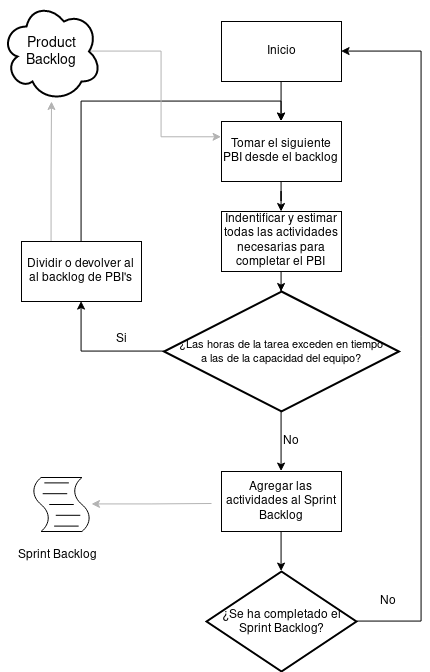
\includegraphics[scale=0.7]{sprintbl.png}
	\centering
	\caption{\label{fig:sprintbacklog} Crear Sprint Backlog}
\end{figure}

Diariamente se llevará una gráfica de Burndown en la que el equipo definirá cuantas horas faltan para acabar el Sprint definido. Así se puede reconocer el progreso del equipo.
\\
\\ Además de lo anterior, se usará un tablero de tareas en una plataforma online (Asana). Se compone de cuatro columnas: en la primera se ven los PBI en orden prioritario definido por el equipo y el ScrumMaster; en la segunda, todas las tareas aún no iniciadas de cada PBI; en la tercera, todas las tareas que estén en progreso y por último, las tareas que ya se han completadas.


% ______________________
% Cap. Product Backlog
% ______________________

\chapter{Product Backlog} 
Los Requerimientos que se asignan como Product Backlog Item son:
\begin{enumerate}
	\item  Entorno de Ventana de Juego
	\item Área de Juego
	\item  Movimiento
	\item Sistema de Puntos
	\item Power-Ups
	\item HUD de Estado del Juego
	\item Perks o Modificadores del Juego
	\item Texturas
	\item Entornos del Juego
	\item Modelos del Juego
	\item Personajes (Snakes)
	\item Otros Entornos
	\item Animaciones
	\item Sonido y Música
\end{enumerate}

\section{Entorno de Ventana de Juego}
Se debe realizar una ventana en la que se pueda realizar el dibujado completo del juego. Esta ventana es el contenedor general de la aplicación y debe cumplir con ciertos requerimientos.

\subsection{Requerimientos}
\begin{itemize}
	\item La ventana debe tener como mínimo $640px$ x $480px$.
	\item La ventana debe adaptarse a la resolución de la pantalla de acuerdo al cambio de la resolución nativa.
	\item En caso de que se ejecute el juego en modo ventana, este debe adaptarse al escalado del usuario.
\end{itemize}

\subsection{Análisis de Contexto}
\subsubsection{Entradas}
\textbf{Modo Pantalla Completa}
\begin{itemize}
	\item Ancho de pantalla nativa en $px$
	\item Alto de pantalla nativa en $px$
\end{itemize}
\textbf{Modo Pantalla}
\begin{itemize}
	\item Ancho de pantalla actual en $px$
	\item Alto de pantalla actual en $px$
\end{itemize}
\subsubsection{Salidas}
La salida debe ser una ventana a pantalla completa dentro de los límites definidos por las entradas nativas. Por otro lado, si no es pantalla completa debe generar una pantalla con las dimensiones especificadas por las dimensiones actuales de la ventana.

%-+-+-+-+-+-+-+-+-+-+-+-+-+-+-+-+-+-+-+-+-+-+-+-+-+-+-+-+-+-+-+-+-+-+-+-+-+-+-+-+-

\section{Área de Juego}
Debe crearse una zona jugable, también llamada mapa o espacio jugable. Este espacio será donde el jugador puede moverse durante una partida.

\subsection{Requerimientos}
\begin{itemize}
	\item El mapa debe ser finito.
	\item En caso de salir del límite del mapa, el juego debe terminar. No debe permitirse salir al jugador nunca.
	\item Debe ser un un cuadrilátero regular.
	\item Debe ser completamente plano, es decir, no debe tener ninguna inclinación
\end{itemize}

\subsection{Análisis de Contexto}
\subsubsection{Entradas}
\begin{itemize}
	\item Coordenada en tres dimensiones del inicio del plano. 
	\item Coordenada en tres dimensiones del final del plano.
\end{itemize}
\subsubsection{Proceso}
Se deben tomar las dos coordenadas para generar el plano en tres dimensiones.
\subsubsection{Salidas}
Plano donde se establecerá el mapa del jugador dibujado en pantalla con los límites visibles.

%-+-+-+-+-+-+-+-+-+-+-+-+-+-+-+-+-+-+-+-+-+-+-+-+-+-+-+-+-+-+-+-+-+-+-+-+-+-+-+-+-

\section{Movimiento}
El movimiento debe de ser implementado para que el jugador pueda determinar la dirección del Snake. 

\subsection{Requerimientos}
\begin{itemize}
	\item Deben realizarse el movimiento con las flechas del teclado.
	\item El usuario no debe poderse moverse en diagonal al presionar dos teclas.
\end{itemize}

\subsection{Análisis de Contexto}
\subsubsection{Entradas}
\begin{itemize}
	\item Flecha presionada por el jugador.
\end{itemize}
\subsubsection{Proceso}
\begin{enumerate}
	\item Al presionar la flecha se debe reconocer cuál de estas fue presionada
	\item Se debe cambiar la dirección del Snake
	\item El Snake debe seguir el nuevo camino delimitado por el movimiento anterior y el actual.
\end{enumerate}
\subsubsection{Salidas}
Snake debe estar orientado hacia la nueva posición y debe seguir en el camino delimitado hasta que se presione de nuevo una tecla (flecha).

%-+-+-+-+-+-+-+-+-+-+-+-+-+-+-+-+-+-+-+-+-+-+-+-+-+-+-+-+-+-+-+-+-+-+-+-+-+-+-+-+-

\section{HUD (Heads-Up Display) - Estado del Juego}
Debe crearse una zona jugable, también llamada mapa o espacio jugable. Este espacio será donde el jugador puede moverse durante una partida.

\subsection{Requerimientos}
\begin{itemize}
	\item Debe llevar la cuenta de los puntos adquiridos.
	\item Permite visualizar los power-ups activos.
	\item Permite visualizar los power-ups disponibles.
	\item No debe entorpecer la visibilidad o la jugabilidad.
\end{itemize}

\subsection{Análisis de Contexto - HUD Puntos}
\subsubsection{Entradas}
\begin{itemize}
	\item Cantidad actualizada de Puntos.
\end{itemize}
\subsubsection{Proceso}
\begin{enumerate}
	\item Se muestra en el HUD la nueva cantidad de puntos.
\end{enumerate}
\subsubsection{Salidas}
Refresco en el HUD de la cantidad de puntos.

\subsection{Análisis de Contexto - HUD Power-Ups Activos}
\subsubsection{Entradas}
\begin{itemize}
	\item Evento Power-Up Activo.
\end{itemize}
\subsubsection{Proceso}
\begin{enumerate}
	\item Se muestra en el HUD el power-up activo de forma distintiva.
\end{enumerate}
\subsubsection{Salidas}
Refresco en el HUD de los power-ups activos.

\subsection{Análisis de Contexto - HUD Power-Ups Disponibles}
\subsubsection{Entradas}
\begin{itemize}
	\item Cantidad actualizada de Puntos.
\end{itemize}
\subsubsection{Proceso}
\begin{enumerate}
	\item Se muestra en el HUD la nueva cantidad de puntos.
\end{enumerate}
\subsubsection{Salidas}
Refresco en el HUD de la cantidad de puntos.


%-+-+-+-+-+-+-+-+-+-+-+-+-+-+-+-+-+-+-+-+-+-+-+-+-+-+-+-+-+-+-+-+-+-+-+-+-+-+-+-+-

\section{Sistema de Puntos}
El sistema de puntos maneja cuantos puntos se da al usuario cuando cumple una acción determinada.

\subsection{Requerimientos}
\begin{itemize}
	\item El sistema de puntos iniciará en 0.
	\item Debe reconocerse la acción que le da puntos al usuario.
	\item Debe mantenerse y protegerse el puntaje para que no sea modificado.
\end{itemize}

\subsection{Análisis de Contexto - Punto Normal (Comida)}
\subsubsection{Entradas}
\begin{itemize}
	\item El jugador ha comido una comida general. Es decir, ha pasado la cabeza de Snake por la comida.
\end{itemize}
\subsubsection{Proceso}
\begin{enumerate}
	\item Se verifica que la cabeza de Snake esté en la misma coordenada que la comida
	\item Se activa el evento de que el usuario pasado por una comida general.
	\item El sistema debe sumar 10 puntos al Puntaje de la partida.
	\item El Puntaje de la Partida debe actualizarse en la pantalla.
	\item Debe aumentar el tamaño de la serpiente en una unidad definida.
\end{enumerate}
\subsubsection{Salidas}
Puntaje general actualizado.

\subsection{Análisis de Contexto - Punto (Mango)}
\subsubsection{Entradas}
\begin{itemize}
	\item El jugador ha comido un "Mango". Es decir, ha pasado la cabeza de Snake por el objeto de juego "Mango".
\end{itemize}
\subsubsection{Proceso}
\begin{enumerate}
	\item Se verifica que la cabeza de Snake esté en la misma coordenada que el objeto "mango".
	\item Se activa el evento de que el usuario pasado por un "mango".
	\item El sistema debe sumar 50 puntos al Puntaje de la partida.
	\item El Puntaje de la Partida debe actualizarse en la pantalla.
	\item Se debe ejecutar el evento de Power-Up Mango. (Ver Análisis de Contexto - PowerUps - Mango)
\end{enumerate}
\subsubsection{Salidas}
Puntaje general actualizado.

\subsection{Análisis de Contexto - Punto (Guaraná)}
\subsubsection{Entradas}
\begin{itemize}
	\item El jugador ha comido un "Guaraná". Es decir, ha pasado la cabeza de Snake por el objeto de juego "Guaraná".
\end{itemize}
\subsubsection{Proceso}
\begin{enumerate}
	\item Se verifica que la cabeza de Snake esté en la misma coordenada que el objeto "Guaraná".
	\item Se activa el evento de que el usuario pasado por un "guaraná".
	\item El sistema debe sumar 80 puntos al Puntaje de la partida.
	\item El Puntaje de la Partida debe actualizarse en la pantalla.
	\item Se debe ejecutar el evento de Power-Up Guaraná. (Ver Análisis de Contexto - PowerUps - Guaraná)
\end{enumerate}
\subsubsection{Salidas}
Puntaje general actualizado.

\subsection{Análisis de Contexto - Punto (Fruto Antiguo)}
\subsubsection{Entradas}
\begin{itemize}
	\item El jugador ha comido un "Fruto Antiguo". Es decir, ha pasado la cabeza de Snake por el objeto de juego "Fruto Antiguo".
\end{itemize}
\subsubsection{Proceso}
\begin{enumerate}
	\item Se verifica que la cabeza de Snake esté en la misma coordenada que el objeto "Fruto Antiguo".
	\item Se activa el evento de que el usuario pasado por un "Fruto Antiguo".
	\item El sistema debe sumar 100 puntos al Puntaje de la partida.
	\item El Puntaje de la Partida debe actualizarse en la pantalla.
	\item Se debe ejecutar el evento de Power-Up Fruto Antiguo. (Ver Análisis de Contexto - PowerUps - Fruto Antiguo)
\end{enumerate}
\subsubsection{Salidas}
Puntaje general actualizado.

%-+-+-+-+-+-+-+-+-+-+-+-+-+-+-+-+-+-+-+-+-+-+-+-+-+-+-+-+-+-+-+-+-+-+-+-+-+-+-+-+-

\section{Power-Ups}
El usuario debe tener la posibilidad de tener modificadores del juego que aumenten la dinámica de este. Estos \emph{Power-Ups} tienen diferentes implicaciones en el juego; es decir, no todos tienen los mismos efectos en la jugabilidad.
\subsection{Requerimientos}
\begin{itemize}
	\item Deben de tener una forma de diferenciarse (Texturas).
	\item Deben modificar la jugabilidad.
	\item Debe tener un forma de saber que están disponibles (HUD, deseable).
	\item Deben tener un tiempo determinado de uso.
\end{itemize}

\subsection{Análisis de Contexto - Power-Up (Mango)}
\subsubsection{Entradas}
\begin{itemize}
	\item Llamada de Evento de Punto (Mango)
\end{itemize}
\subsubsection{Proceso}
\begin{enumerate}
	\item Se activa el evento Mango.
	\item El HUD tendrá un indicador con el tiempo faltante para que acabe el efecto del power-up
	\item El puntaje parcial adquirido durante el tiempo tendrá un multiplicador.
	\item Se genera de manera aleatoria el multiplicador utilizando un generador de números pseudoaleatorios (GPAN) de Mersenne Twister.
	\item Se asigna el multiplicador
	\item Al cumplir el tiempo, el multiplicador debe ser retirado.
\end{enumerate}
\subsubsection{Salidas}
Power-Up Mango activado.

\subsection{Análisis de Contexto - Power-Up (Guaraná)}
\subsubsection{Entradas}
\begin{itemize}
	\item Llamada de Evento de Punto (Guaraná)
\end{itemize}
\subsubsection{Proceso}
\begin{enumerate}
	\item Se activa el evento Guaraná.
	\item El HUD tendrá un indicador con el tiempo faltante para que acabe el efecto del power-up
	\item La velocidad de Snake se verá afectada en un porcentaje aleatorio.
	\item Se genera de manera aleatoria el porcentaje de incremento de velocidad utilizando un generador de números pseudoaleatorios (GPAN) de Mersenne Twister.
	\item Se asigna el porcentaje
	\item Al cumplir el tiempo, el multiplicador debe ser retirado.
\end{enumerate}
\subsubsection{Salidas}
Power-Up Guaraná activado con velocidad incrementada en el movimiento de Snake.

\subsection{Análisis de Contexto - Power-Up (Fruto Antiguo)}
\subsubsection{Entradas}
\begin{itemize}
	\item Llamada de Evento de Punto (Fruto Antiguo)
\end{itemize}
\subsubsection{Proceso}
\begin{enumerate}
	\item Se activa el evento Fruto Antiguo.
	\item El HUD tendrá un indicador con el tiempo faltante para que acabe el efecto del power-up
	\item Se añadirá la posibilidad de "renacer" si Snake está en uno de los Fin de Juego (exceptuando máximo puntaje).
	\item Se asigna el poder de resurrección para ser usado.
\end{enumerate}
\subsubsection{Salidas}
Power-Up Fruto Antiguo Activado y asignado fruto antiguo en el HUD.

%-+-+-+-+-+-+-+-+-+-+-+-+-+-+-+-+-+-+-+-+-+-+-+-+-+-+-+-+-+-+-+-+-+-+-+-+-+-+-+-+-

\section{Entornos del Juego}
Se deben realizar dos niveles diferentes que sean jugables.
\subsection{Requerimientos}
\begin{itemize}
	\item El primero debe ser un lugar simple con muros al estilo laberinto. Similar a un laboratorio de experimentación.
	\item El segundo debe intentar reproducir un entorno salvaje con diferentes objetos que lo permitan, e.g. piedras, árboles, agua y vegetación variada.
\end{itemize}

%-+-+-+-+-+-+-+-+-+-+-+-+-+-+-+-+-+-+-+-+-+-+-+-+-+-+-+-+-+-+-+-+-+-+-+-+-+-+-+-+-

\section{Modelos del Juego}
Es necesario reproducir de la forma más fiel posible la serpiente y la forma que tiene. 
\subsection{Requerimientos}
\begin{itemize}
	\item Debe representar la forma de una serpiente. Esto puede ser un cilindro alargado que crece con el tiempo.
	\item Sin embargo, se debe dejar de un ancho fijo para que se puedan aplicar las texturas en un futuro de forma sencilla.
\end{itemize}

%-+-+-+-+-+-+-+-+-+-+-+-+-+-+-+-+-+-+-+-+-+-+-+-+-+-+-+-+-+-+-+-+-+-+-+-+-+-+-+-+-

\section{Personajes (Snakes)}
Se pretende implementar otras serpientes con caracteristicas diferentes. La única diferencia es la textura aplicada.
\subsection{Requerimientos}
\begin{itemize}
	\item Python
	\item Mamba
\end{itemize}


%-+-+-+-+-+-+-+-+-+-+-+-+-+-+-+-+-+-+-+-+-+-+-+-+-+-+-+-+-+-+-+-+-+-+-+-+-+-+-+-+-

\section{Animaciones}
Implementar animaciones que mejoren el aspecto visual del juego.
\subsection{Requerimientos}
\begin{itemize}
	\item Animación de comida para representar cuando cada uno de las serpientes come.
	\item Animación de Power-Ups para representar cuando se adquiere o se usa un Power-Up
\end{itemize}

%-+-+-+-+-+-+-+-+-+-+-+-+-+-+-+-+-+-+-+-+-+-+-+-+-+-+-+-+-+-+-+-+-+-+-+-+-+-+-+-+-

\section{Sonido y Música}
Se deben incluir archivos de audio que mejoren el aspecto auditivo del juego.
\subsection{Requerimientos}
\begin{itemize}
	\item Sonidos aleatorios de la serpiente.
	\item Música de Introducción
	\item Música de Entornos
	\item Sonido de uso de Power-Ups
	\item Sonido de Comida
	\item Sonido de Final del Juego
\end{itemize}


%-+-+-+-+-+-+-+-+-+-+-+-+-+-+-+-+-+-+-+-+-+-+-+-+-+-+-+-+-+-+-+-+-+-+-+-+-+-+-+-+-

\section{Texturas}
Es necesario incluir texturas que permitan darle más realismo al juego. En este caso, para los personajes, objetos y entornos.

\subsection{Requerimientos}
\begin{itemize}
	\item Las texturas deben ser acordes y fieles a la representación en el mundo real.
	\item En lo posible, deben ser lo más ligeras posibles sin sacrificar la calidad.
\end{itemize}



% ______________________
% Cap. Herramientas y Servicios
% ______________________

\chapter{Herramientas y Servicios}

\section{Compilación y Lenguaje}

Se utilizará OpenGL en C++. Las versiones respectivas instaladas de base son:

\begin{itemize}

	\item g++ (Arch 9.1.0) 9.1.0

	\item GNU gdb gbd-common-8.3-1

	\item Clang 8.0.1-1

	\item make 4.2.1-3

	\item CMake 3.15.2

\end{itemize}
\section{Integración Continua (CI) y Manejo de Versiones}
Se deben utilizar manejo de versiones e integración continua que permitan la verificación de calidad de los commits realizados en cada sprint. Gracias a esto es posible manejar las versiones y encontrar problemas en un menor tiempo.
Las herramientas utilizadas para este proyecto serán: 
\begin{itemize}
	 \item Travis CI Ubuntu 16.04 Xenial Xerus LTS, 18.04 Bionic Beaver LTS
	 \item git 2.23.0
	 \item GitKraken 6
\end{itemize}
% ______________________
% Cap. Mundo / Entorno de Juego
% ______________________
\chapter{Mundo / Entorno de Juego}

\section{Laboratorio}
El laboratorio es un lugar completamente blanco representando un laberinto de pruebas. Se debe ver como una caja delimitada por el área de juego con paredes color blanco. Debe tener obstáculos en forma de paredes.

\section{Jungla}
Jungla debe representar un ambiente natural de jungla. En este, para mayor facilidad se debe buscar que sea un campo abierto sin demasiados obstáculos y que se pueda ver en los límites la jungla como si fueran las paredes.

% ______________________
% Cap. Pantallas de Juego
% ______________________
\chapter{Pantallas de Juego}
Las pantallas de juego deben realizarse para orientar al usuario e iniciar nuevos juego o indicar el final de estos.

\section{Pantalla de Inicio}
Debe ser una pantalla donde se encuentre el logo del juego en la parte superior. Un texto en el que se indiquen las instrucciones para iniciar un nuevo juego y a la izquierda un scoreboard con los puntajes más altos. En la parte baja de la pantalla se ubica la version de la build del juego y el copyright.

\section{Menu}
Debe permitir elegir los escenarios y la serpiente con la que se quiere jugar. 

\section{Fin de Juego}
Muestra la leyenda de "Fin de Juego", la puntación obtenida y si esta es un nuevo récord, la opción para comenzar de nuevo y la opción para salir a la pantalla de Inicio.


% ______________________
% Cap. Controles
% ______________________
\chapter{Controles}
Los controles son en un teclado de cualquier distribución con caracteres latinos.
\begin{figure}
[h]
	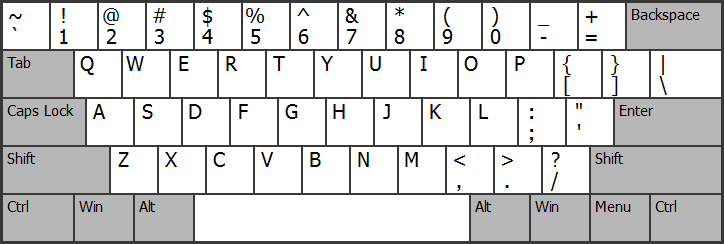
\includegraphics[scale=0.7]{layout.png}
	\centering
	\caption{\label{fig:sprintbacklog} Layout US. Ejemplo de Teclado con Distribución Latina. Tomado de:  wikipedia.org}
\end{figure}
\section{Movimiento}
Se usan las flechas del teclado.
\section{Power-Ups}
Se usan Q, W, E para activar los Power-Ups ( Mango, Guaraná y Fruto Antiguo respectivamente).



% ______________________
% Cap. Geometría de Entornos y Personajes
% ______________________
\chapter{Geometría de Entornos, Personajes y Objetos}
\section{Entornos}
Los entornos serán delimitados dentro de una caja definida dentro de los límites del área de juego.
\section{Personajes}
Las serpientes tendrán forma alargada cilíndrica. Todas tendrán el mismo diámetro para facilitar la aplicación de las texturas.
\section{Power-Ups}
Los Power-Ups tendrán diferentes formas:
\subsection{Comida General}
Será una caja cuadrada color rojo, similar al color de la carne.
\subsection{Mango}
Representado por una esfera de color amarillo y diferentes gamas del naranja.
\subsection{Guaraná}
Representado por una esfera pequeña de color rojo.
\subsection{Fruto Antiguo}
Representado por una esfera metálica.
% ______________________
% Cap. Gantt y Calendario de Actividades
% ______________________
\chapter{Gantt y Calendario de Actividades}
Se realiza un diagrama de actividades para finalizar el proyecto en el tiempo justo. Cada una tiene el tiempo estimado en días para completarse.
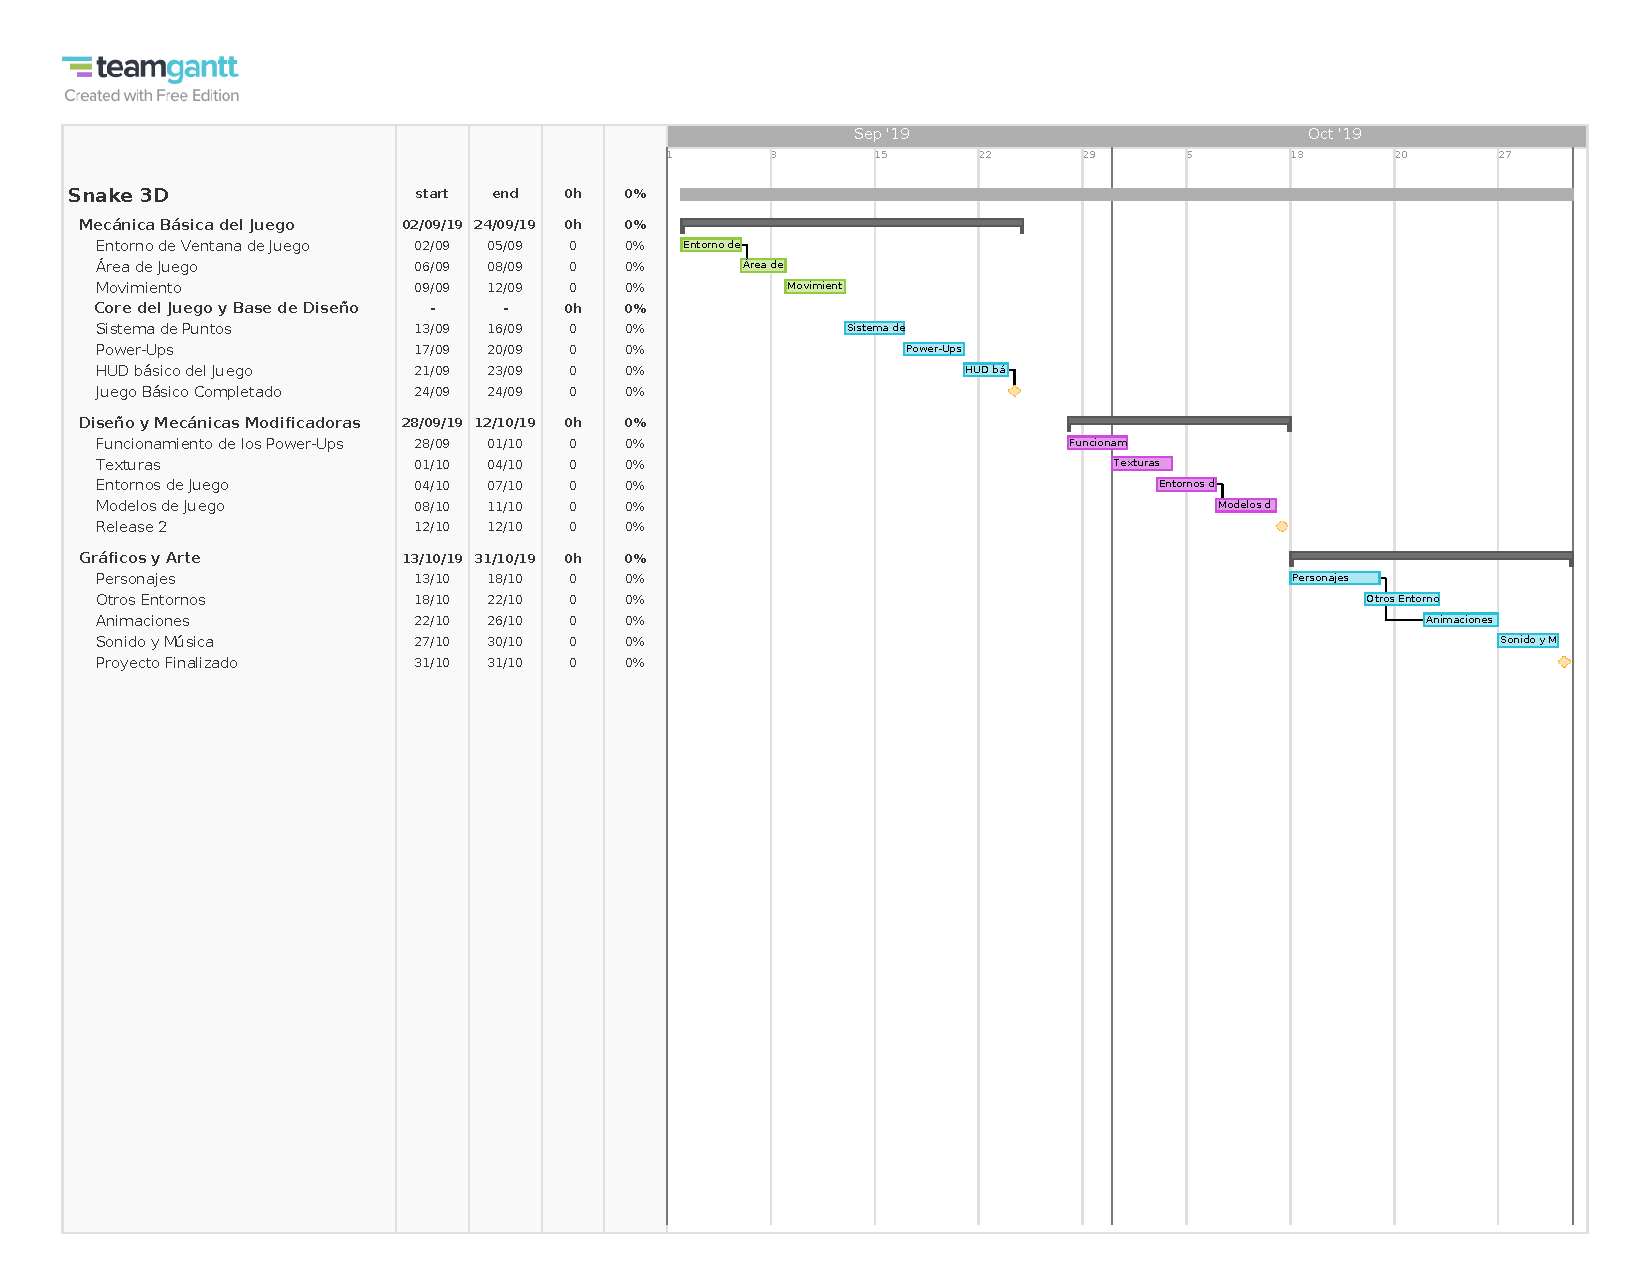
\includepdf{gantt.pdf}
% ______________________
% chapter Game Details
% ______________________
\chapter{Créditos y Bibliografía}


Keith, Clinton.

Agile game development w i t h Scrum / Clinton Keith.

p. cm.

Includes index.

ISBN 0-321-61852-1 (pbk.: alk. paper) 1. C o m p u t e r games—Programming. 2. Agile soft-

ware development. 3. Scrum (Computer software development) I.Title.

QA76.76.C672K45 2010

005.1—dc22


%\todo[inline, color=green!40]{This is an inline comment.}

%\bibliographystyle{alpha}
%\bibliography{sample}

\end{document}